\documentclass[11pt]{article}
\usepackage{sectsty}
\usepackage{graphicx}
\usepackage{caption}
\usepackage{subcaption}
\usepackage{fancyhdr}
\usepackage[section]{placeins} %Prevents placeing floats before a section


% Margins
\topmargin=-0.45in
\evensidemargin=0in
\oddsidemargin=0in
\textwidth=6.5in
\textheight=9.0in
\headsep=0.25in

\title{ DATASCI2G03 Final Project: Modifying a model of Trypanosome Infections to account for Co-infection of the Malaria Parasite  }
\author{ Alexander Turco, TA: Hector Robin  }
\date{\today}

%% Hyperreferecing Biliography
\usepackage[hidelinks, colorlinks=true, linkcolor=blue, citecolor=blue]{hyperref}


%%BIBLIOGRAPHY
\usepackage[natbib=true, sorting=nyt, style = authoryear-comp, sortcites=ynt, maxcitenames=2]{biblatex}
\addbibresource{ABC1.bib}

%%Page style for header
\pagestyle{fancy}
\fancyhf{}
\fancyfoot[C]{\thepage}
%\fancyhead[EL]{\nouppercase\leftmark}
%\fancyhead[OR]{\nouppercase\rightmark}
%\fancyhead[ER,OL]{\thepage}

%%Fun with captions
\usepackage[skip=2pt,font=small]{caption}
\captionsetup[figure]{labelfont={color=blue},font={color=black}, }

%FOR INSERTING CODE
\usepackage{listings}
\usepackage{xcolor}

\definecolor{codegreen}{rgb}{0,0.6,0}
\definecolor{codegray}{rgb}{0.5,0.5,0.5}
\definecolor{codepurple}{rgb}{0.58,0,0.82}
\definecolor{backcolour}{rgb}{0.95,0.95,0.92}

\lstdefinestyle{mystyle}{
	backgroundcolor=\color{backcolour},   
	commentstyle=\color{codegreen},
	keywordstyle=\color{magenta},
	numberstyle=\tiny\color{codegray},
	stringstyle=\color{codepurple},
	basicstyle=\ttfamily\footnotesize,
	breakatwhitespace=false,         
	breaklines=true,                 
	captionpos=b,                    
	keepspaces=true,                 
	numbers=left,                    
	numbersep=5pt,                  
	showspaces=false,                
	showstringspaces=false,
	showtabs=false,                  
	tabsize=2
}

\lstset{style=mystyle}


\begin{document}	
	\maketitle
	\vspace{-1cm}
	\begin{center}
		Student Number: 400235250
	\end{center}
	
	\pagebreak
	
	% Optional TOC
	 \tableofcontents
	 \pagebreak
	
	%--Paper--
	\section{A Brief Background}
	
	Trypanosomes are single celled eukaryotic parasites which maintain a chronic parasitaemia (parasites present in the blood) in a variety of mammalian hosts \citep{tyler2001limitation}. The way in which these Trypanosomes are able to infect mammalian hosts stems from a balance between Trypanosome proliferation, differentiation and cell death \citep{tyler2001limitation}. In a study conducted by \citet{tyler2001limitation}, researchers utilized data pertaining to the number of parasite cells/ml of blood in mice to develop mathematical models which could help to better understand Trypanosome infections.
	
	The way in which the researchers modelled these complex interactions of cell proliferation, differentiation, and cell death was based upon two types of cells that were measured in blood samples obtained from the mice. The first cell type is called 'slender' and these multiply exponentially in the host. The second cell type is 'stumpy' cells and these no longer divide. Slender cells can differentiate into stumpy cells and this is initiated when the cell concentration of these slender cells becomes high \citep{tyler2001limitation}. This differentiation of slender cells to stumpy cells will stop the exponential growth of slender cells and prevent these parasites from killing the host in a quick manner.
	
	To model the slender-to-stumpy cell transition, \citep{tyler2001limitation} utilized differential equations to describe the rate at which the total parasite changes with respect to time. This project will utilize \texttt{C++} to employ a fourth-order Runge-Kutta method that will allow us to find the solution to this set of differential equations. We will compare results to the findings of \citep{tyler2001limitation} to confirm that our model is working as it should, and we will also expand the model to account for co-infection.
	
	
	%%MAYBE ADD MODEL 1 AND MODEL 2 HERE LIKE THE UPDATED EQUATIONS WITH APOPTOSIS OR IMMUNITY VALUES INVOLVED
	\section{Methods}
	
	The concentration of slender and stumpy cells was first proposed by \citep{turner1995replication} using two differential equations, one to model replication of slender cells at density X (1) and one to model the differentiation of slender to stumpy cells at density Y (2).
	
	\begin{equation}
		\frac{dX}{dT} = (r-f)X(t)
	\end{equation}
	
	\begin{equation}
		\frac{dY}{dT} = fX(t)-mY(t)
	\end{equation}\newline
	$X$ is the concentration of slender cells at time t \newline
	$Y$ is the concentration of stumpy cells at time t \newline
	$r$ is the rate of division of slender cells \newline
	$f$ is the rate of differentiation of slender-to-stumpy cells \newline
	$m$ is the mortality rate of stumpy cells \newline
	
	In order to achieve a solution to the differential equations, \citep{tyler2001limitation} modified the model by introducing density dependent trypanosome differentiation. The assumption is made that $f = f_0(X+Y)$ which means that the differentiation rate is proportional to the total population/concentration of both cell types. This can be inserted into the equations above to get two slightly different equations (3) and (4) which are shown below.
	
	\begin{equation}
		\frac{dX}{dT} = (r-f_0(X+Y))X
	\end{equation}
	
	\begin{equation}
		\frac{dY}{dT} = f_0(X+Y)X-mY
	\end{equation}
	Now, these equations are able to be solved by utilizing a fourth-order Runge-Kutta method, in the same way as \citep{tyler2001limitation}. The parameters $r$ and $m$ have already been mentioned above, but $f_0$ and $X_0$ are two parameters that are used to set initial conditions and create a solution using a fourth-order Runge-Kutta method. This method was implemented in \texttt{C++} and in order to see if the system behaved correctly, plots were used to visualize the populations of the two different cell types, as well as the total population of both cell types (X+Y). This study will compare results to those of \citep{tyler2001limitation}, and build upon the model by accounting for co-infection.
	
	\section{Testing the Program}
	
	To test if the initial \texttt{C++} program functioned correctly, the same parameter values used in the study performed by \citep{tyler2001limitation} were used to produce a plot. Below are the results of the comparison. \newline
	
	\begin{figure}[!htb]
		\centering
		\begin{subfigure}{.5\textwidth}
			\centering
			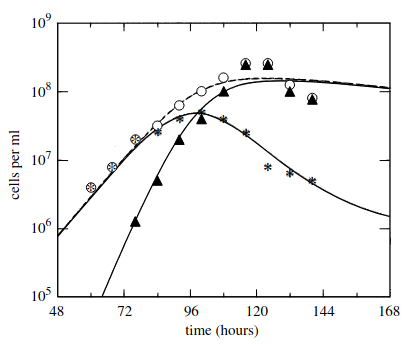
\includegraphics[width=7cm, height=6cm]{plot1.png}
			\caption{Figure taken from \citep{tyler2001limitation}}
			\label{fig:sub1}
		\end{subfigure}%
		\begin{subfigure}{.5\textwidth}
			\centering
			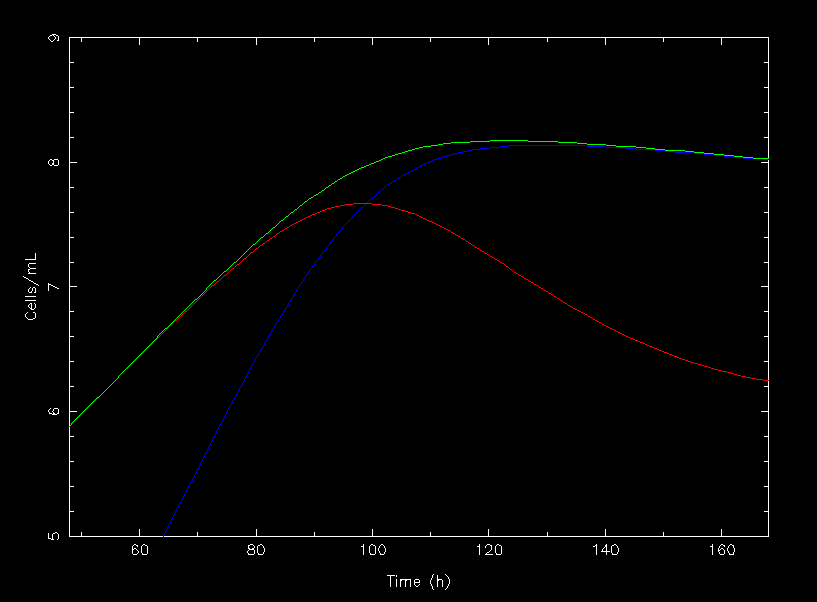
\includegraphics[width=7cm, height=6cm]{plot2.png}
			\caption{Figure made with \texttt{pgplot} by me}
			\label{fig:sub2}
		\end{subfigure}
		\caption{Fitting differential equations (3) and (4) to infected mice with parameters $r = 0.11$, $f_0 = 1.2$ x $10^-9$, $m = 0.012$ and $X_0 = 3.91$ x $10^3$. This figure shows a comparison between the different cell populations over a time period of 168 hours found by \citep{tyler2001limitation} (a) and found by me (b). Both solutions were found using a fourth-order Runge-Kutta method. The green line represents the total trypanosome concentration, the red line represents the concentration of slender cells and the blue line represents the concentration of stumpy cells. In Figure (a) the circles, stars, and triangles are representative of data the researchers obtained from the mice, pertaining to the total trypanosome concentration, slender cell concentration, and stumpy cell concentration respectively. These findings suggest that first of all this is an accurate model and second of all the \texttt{C++} program works.}
		\label{fig:test}
	\end{figure}


	\begin{figure}[!htb]
		\centering
		\begin{subfigure}{.5\textwidth}
			\centering
			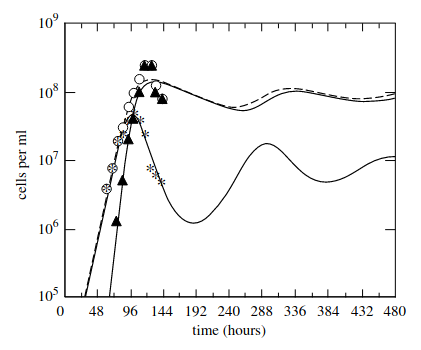
\includegraphics[width=7cm, height=6cm]{plot3.png}
			\caption{Figure taken from \citep{tyler2001limitation}}
			\label{fig:sub1}
		\end{subfigure}%
		\begin{subfigure}{.5\textwidth}
			\centering
			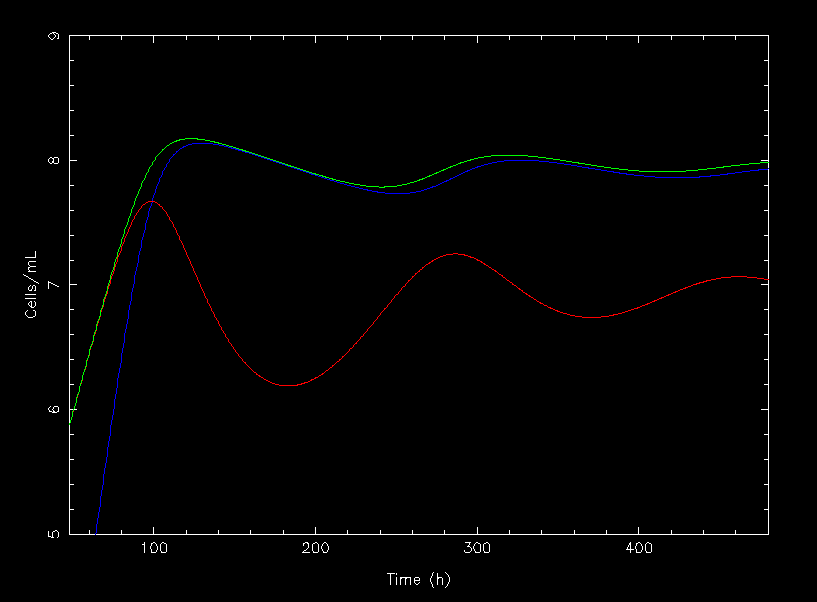
\includegraphics[width=7cm, height=6cm]{plot4.png}
			\caption{Figure made with \texttt{pgplot} by me}
			\label{fig:sub2}
		\end{subfigure}
		\caption{Fitting differential equations (3) and (4) to infected mice with parameters $r = 0.11$, $f_0 = 1.2$ x $10^-9$, $m = 0.012$ and $X_0 = 3.91$ x $10^3$. This figure shows a comparison between the different cell populations over a time period of 480 hours found by \citep{tyler2001limitation} (a) and found by me (b). These plots are essentially continuations of the theoretical curves from Figure 1 and the oscillations in trypanosome concentration in all three lines provides good evidence of density dependent differentiation as we can see slender cells differentiate to stumpy cells when the concentrations of slender cells reach a high concentration. The matching of results also further confirms the \texttt{C++} program I wrote is running correctly.}
		\label{fig:test}
	\end{figure}
	
	\section{Results and Extensions}
	
	An excellent way to modify/extend this model is to consider the effects of the immune repsonse, which is something that \citet{tyler2001limitation} have already done. In section (4.1). To try something new, I want to modify the model proposed by \citet{tyler2001limitation} by accounting for co-infection. In a given host, pathogens are rarely found in isolation, meaning they interact with each other and potentially affect the composition of other bacteria \citep{venter2022parasite}. A study performed by \citet{sanches2019trypanosoma} reported that \textit{T. brucei} infection can actually protect mice from \textit{P. berghei} infection (malaria).
	
	\subsection{Co-infection Model}
	Upon modifying this system, we now have 3 equations.
	
	\begin{equation}
		\frac{dX}{dT} = (r-f_0(X+Y))X
	\end{equation}
	
	\begin{equation}
		\frac{dY}{dT} = f_0(X+Y)X-mY
	\end{equation}

	\begin{equation}
		\frac{dC}{dT} = (r_2 -f_0(X+Y))X-mY-m_2C
	\end{equation}
	$C$ is the concentration of malaria causing cells at time t \newline
	$r_2$ is the rate of division of malaria causing cells \newline
	$m_2$ is the mortality rate of malaria cells\newline	
	
	
	To not over-complicate the model the assumption is once again made that $f = f_0(X+Y)$. In this modified model, I developed a third equation (7) to model the population/concentration of \textit{Plasmodium berghei} which causes malaria. I modelled this equation based off the findings from \citet{sanches2019trypanosoma} which suggest that a Trypanosome infection can provide protection against malaria infections. New parameters I introduced are $r_2$ and $m_2$ and $C$.
	
	\subsection{Results Using Parameters $r = 0.11$, $r_2 = 0.20$, $m = 0.012$, $m_2 = 0.02$, $f_0 = 1.2e-9$, $X_0 = 3910.00$, $Y_0= 1e-10$, $C_0= 3.91e9$}
	
	\begin{figure}[!htb]
		\begin{center}
		\begin{subfigure}{8cm}
			\centering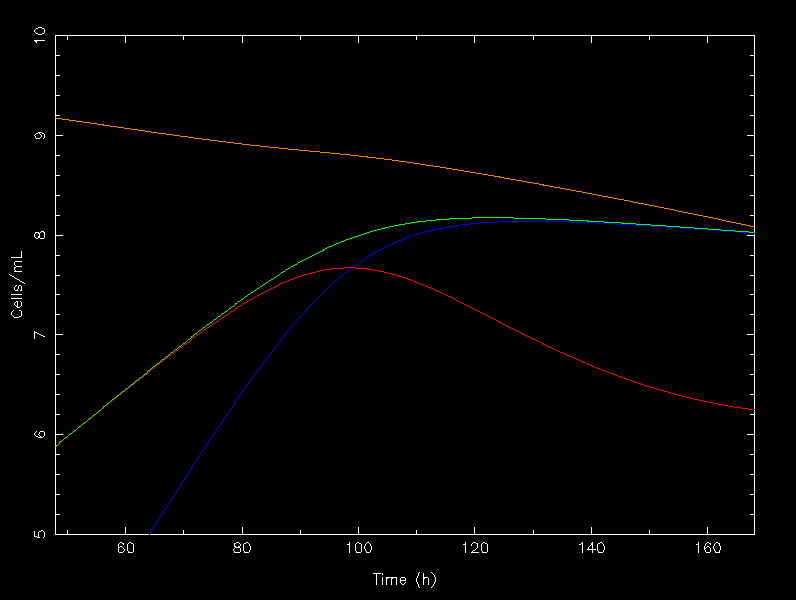
\includegraphics[width=6cm, height=5cm]{plot6.png}
			\caption{Figure made with \texttt{pgplot} by me (168h)}
		\end{subfigure}
		\begin{subfigure}{8cm}
			\centering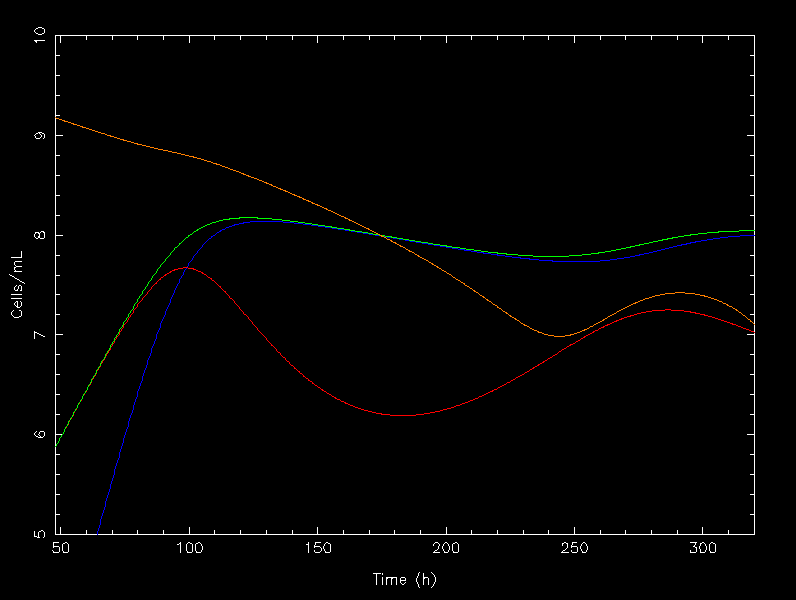
\includegraphics[width=6cm, height=5cm]{plot5.png}
			\caption{Figure made with \texttt{pgplot} by me (300h)}
		\end{subfigure}
			\begin{subfigure}{8cm}
				\centering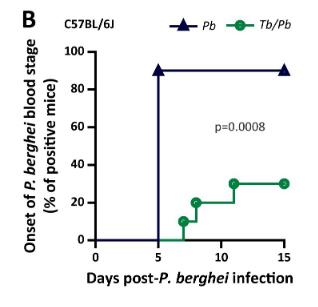
\includegraphics[width=6cm, height=5cm]{plot7.png}
				\caption{Figure taken from \citep{sanches2019trypanosoma}}
			\end{subfigure}
			\begin{subfigure}{8cm}
				\centering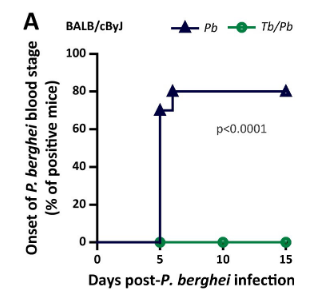
\includegraphics[width=6cm, height=5cm]{plot8.png}
				\caption{Figure taken from \citep{sanches2019trypanosoma}}
			\end{subfigure}
		\caption{This figure reveals similarities in the findings of my expanded model, and real data collected from mice by \citet{sanches2019trypanosoma}. Figures (c) and (d) show the percentage of mice displaying \textit{Plasmodium berghei} parasitaemia, measured by flow cytometry. The black line represents those who were innoculated with \textit{P. berghei} and the green line represents those innoculated with \textit{P. berghei} after being infected with \textit{T. brucei} (trypanosome) five days earlier. It is clear to see the significant differences between the lower number of mice that have parasitaemia and a were infected with trypanosomes prior to malaria innculation, and the higher number of mice who were that have parasitemia and were infected by malaria cells only. Figures (a) and (b) were produced by me and the orange line represents the theoretical concentration of \textit{P. berghei}. What is important to notice is the initial decrease in the concentration of \textit{P. berghei} as the total concentration of slender and stumpy cells (green line) remains fairly consistent. Figure (b) shows the concentrations over 300h and from these results we can see clearly the population of malaria causing cells decreasing, but we also see it increase for a little as the population of slender cells increase.}
		\end{center}
	\end{figure}

	\section{Conclusions and Future Work}
	
	Overall, the findings of this study provide further evidence for a role played by Trypanosomes in the prevention of malaria infection. Utilizing past studies, I developed a modified system of differential equations to model a trypanosome infection and account for the addition of another bacterial population known to commonly co-infect hosts who also have Trypanosomes present. \textit{P. berghei} causes malaria in its host but it has been found that upon co-infection, Trypanosomes suppress the effects of the malaria causing cells. The equation I added to account for this new population of malaria causing cells is based on the same assumptions used by \citet{tyler2001limitation}. The results from this theoretical model do show a decrease in the concentration of malaria causing cells over time, but it is also interesting to note the relationship between the curve of slender cells and the curve of \textit{P. berghei} cells. As the concentration of slender cells rises after reaching a low point, so does the concentration of malaria causing cells.
	
	It would be extremely interesting  to take this model even further to explore the reason why the presence of Trypanosomes impacts the presence of malaria cells. Does the immune system have anything to do with it? Should we account for spontaneous cell death? There are so many biological questions to explore and so many parameters we can incorporate into this model to get a more accurate representation of how this process actually works.
	
	\newpage
	
	%%%Good way to get bibliography as a section in biblatex
	\section{References}
	\printbibliography[
	heading=none
	]
	\newpage
	
	\section{\texttt{C++} Code}
	
	\texttt{trypanosomes.cpp}
	\lstinputlisting[language=c++]{code/trypanosomes.cpp}
	\newpage
	\texttt{functions.cpp}
	\lstinputlisting[language=c++]{code/functions.cpp}
	\texttt{Makefile}
	\lstinputlisting[language=c++]{code/Makefile}
	
	
	
\end{document}